\titleformat{\chapter}
{\normalfont\fontsize{12}{15}\centering}{Anexos \thechapter.}{0.3em}{}[]

\clearpage
\thispagestyle{empty}
\begin{center}
  \vspace*{\fill}
  \phantomsection
  Apéndices
  \addcontentsline{toc}{chapter}{Anexos}
  \vspace*{\fill}
\end{center}
\clearpage

\appendix
% \uextra{Apendice}{Dispositivo Raspberry Pi 4 Model B}
% \begin{figure}[ht!]
%   \centering
%   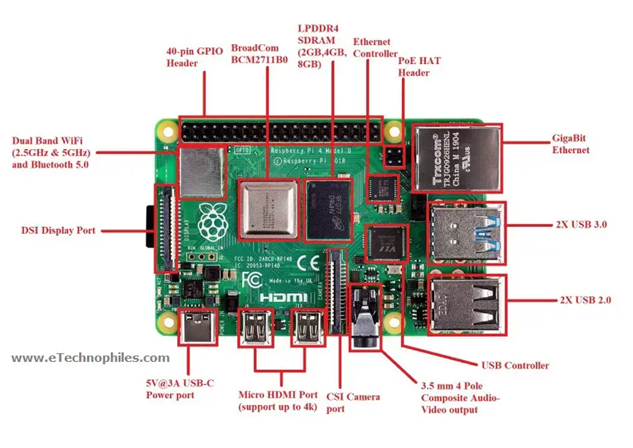
\includegraphics[width=0.95\textwidth]{Anexos/1.arquitectura-raspberry.png}
%   \caption{Arquitectura del Raspberry Pi 4 Model B}
%   \label{fig:raspberry-architecture}
% \end{figure}

\uextra{Apendice}{Representación cíclica del tiempo mediante funciones trigonométricas}
\begin{figure}[ht!]
  \centering
  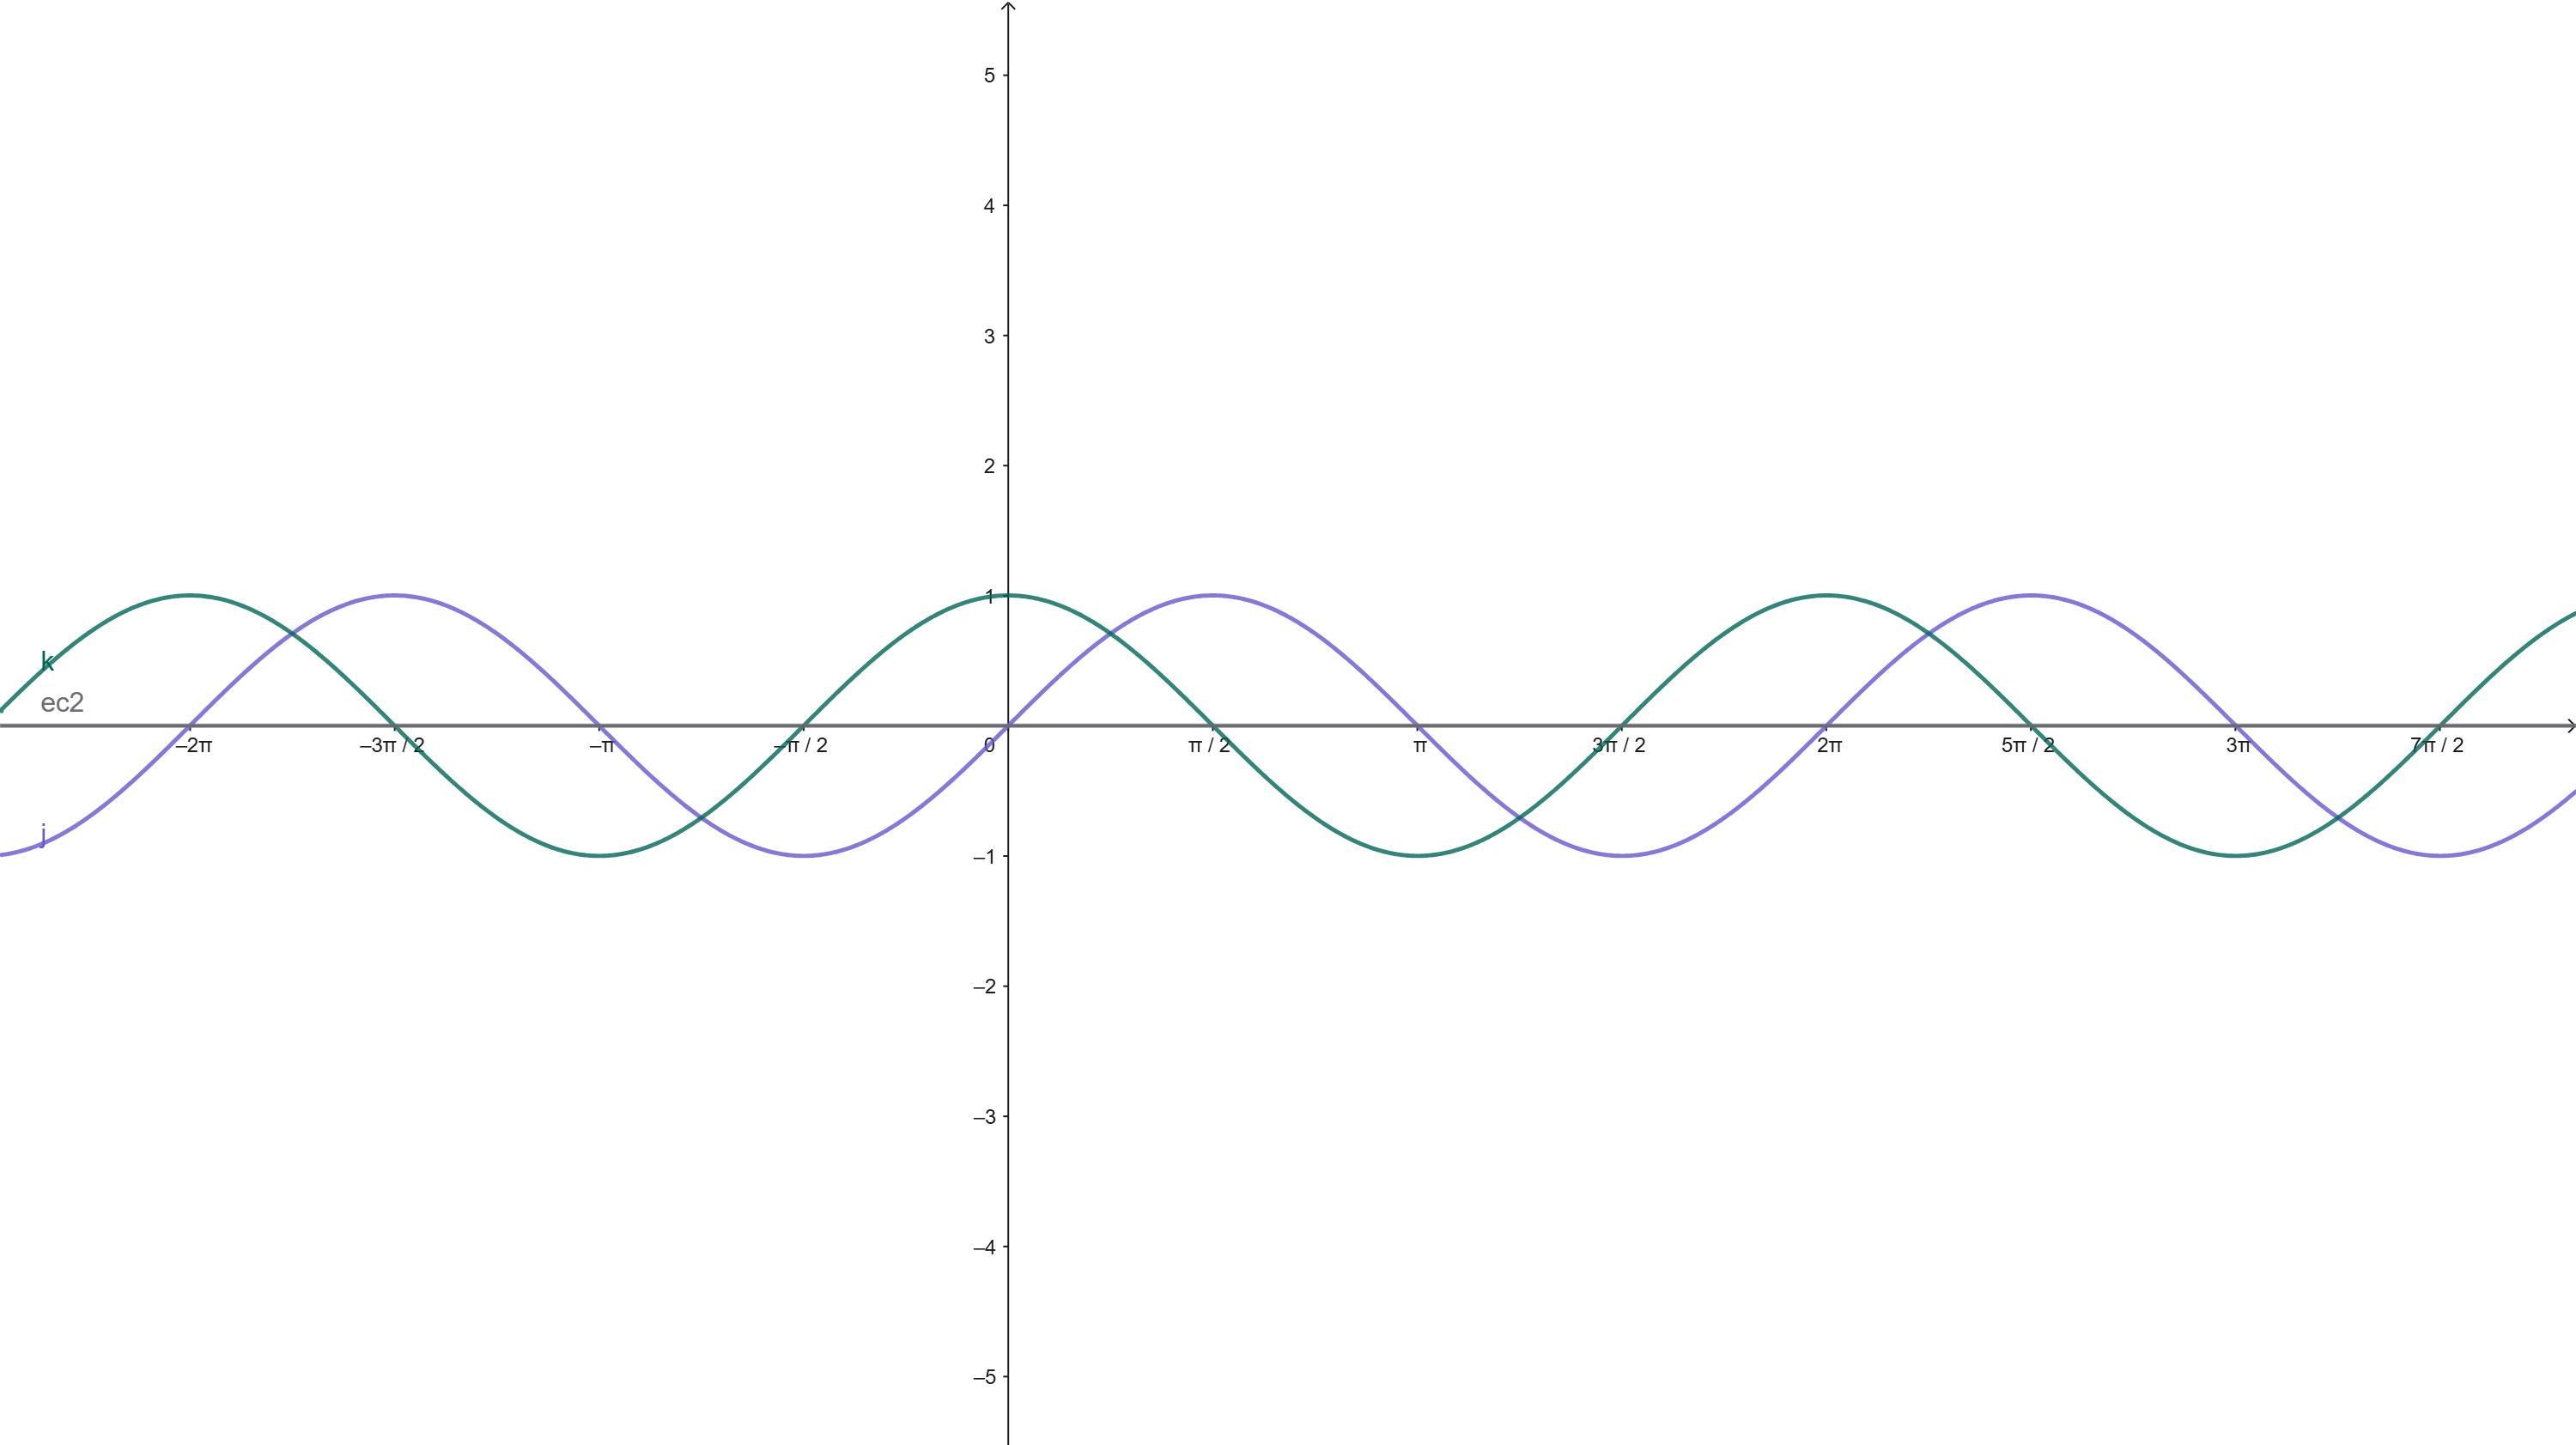
\includegraphics[width=0.55\textwidth]{Apendices/sencos.png}
  \caption{Visualización de las funciones seno y coseno  }
  \caption*{GeoGebra: Generación de las funciones seno y coseno usando las expresiones: \newline
    \texttt{Sequence((x, sin(x)), x, 0, 2$\pi$, $\pi$/6)} y \newline
    \texttt{Sequence((x, cos(x)), x, 0, 2$\pi$, $\pi$/6)}}
  \label{fig: seno-coseno}
\end{figure}
\begin{figure}[ht!]
  \centering
  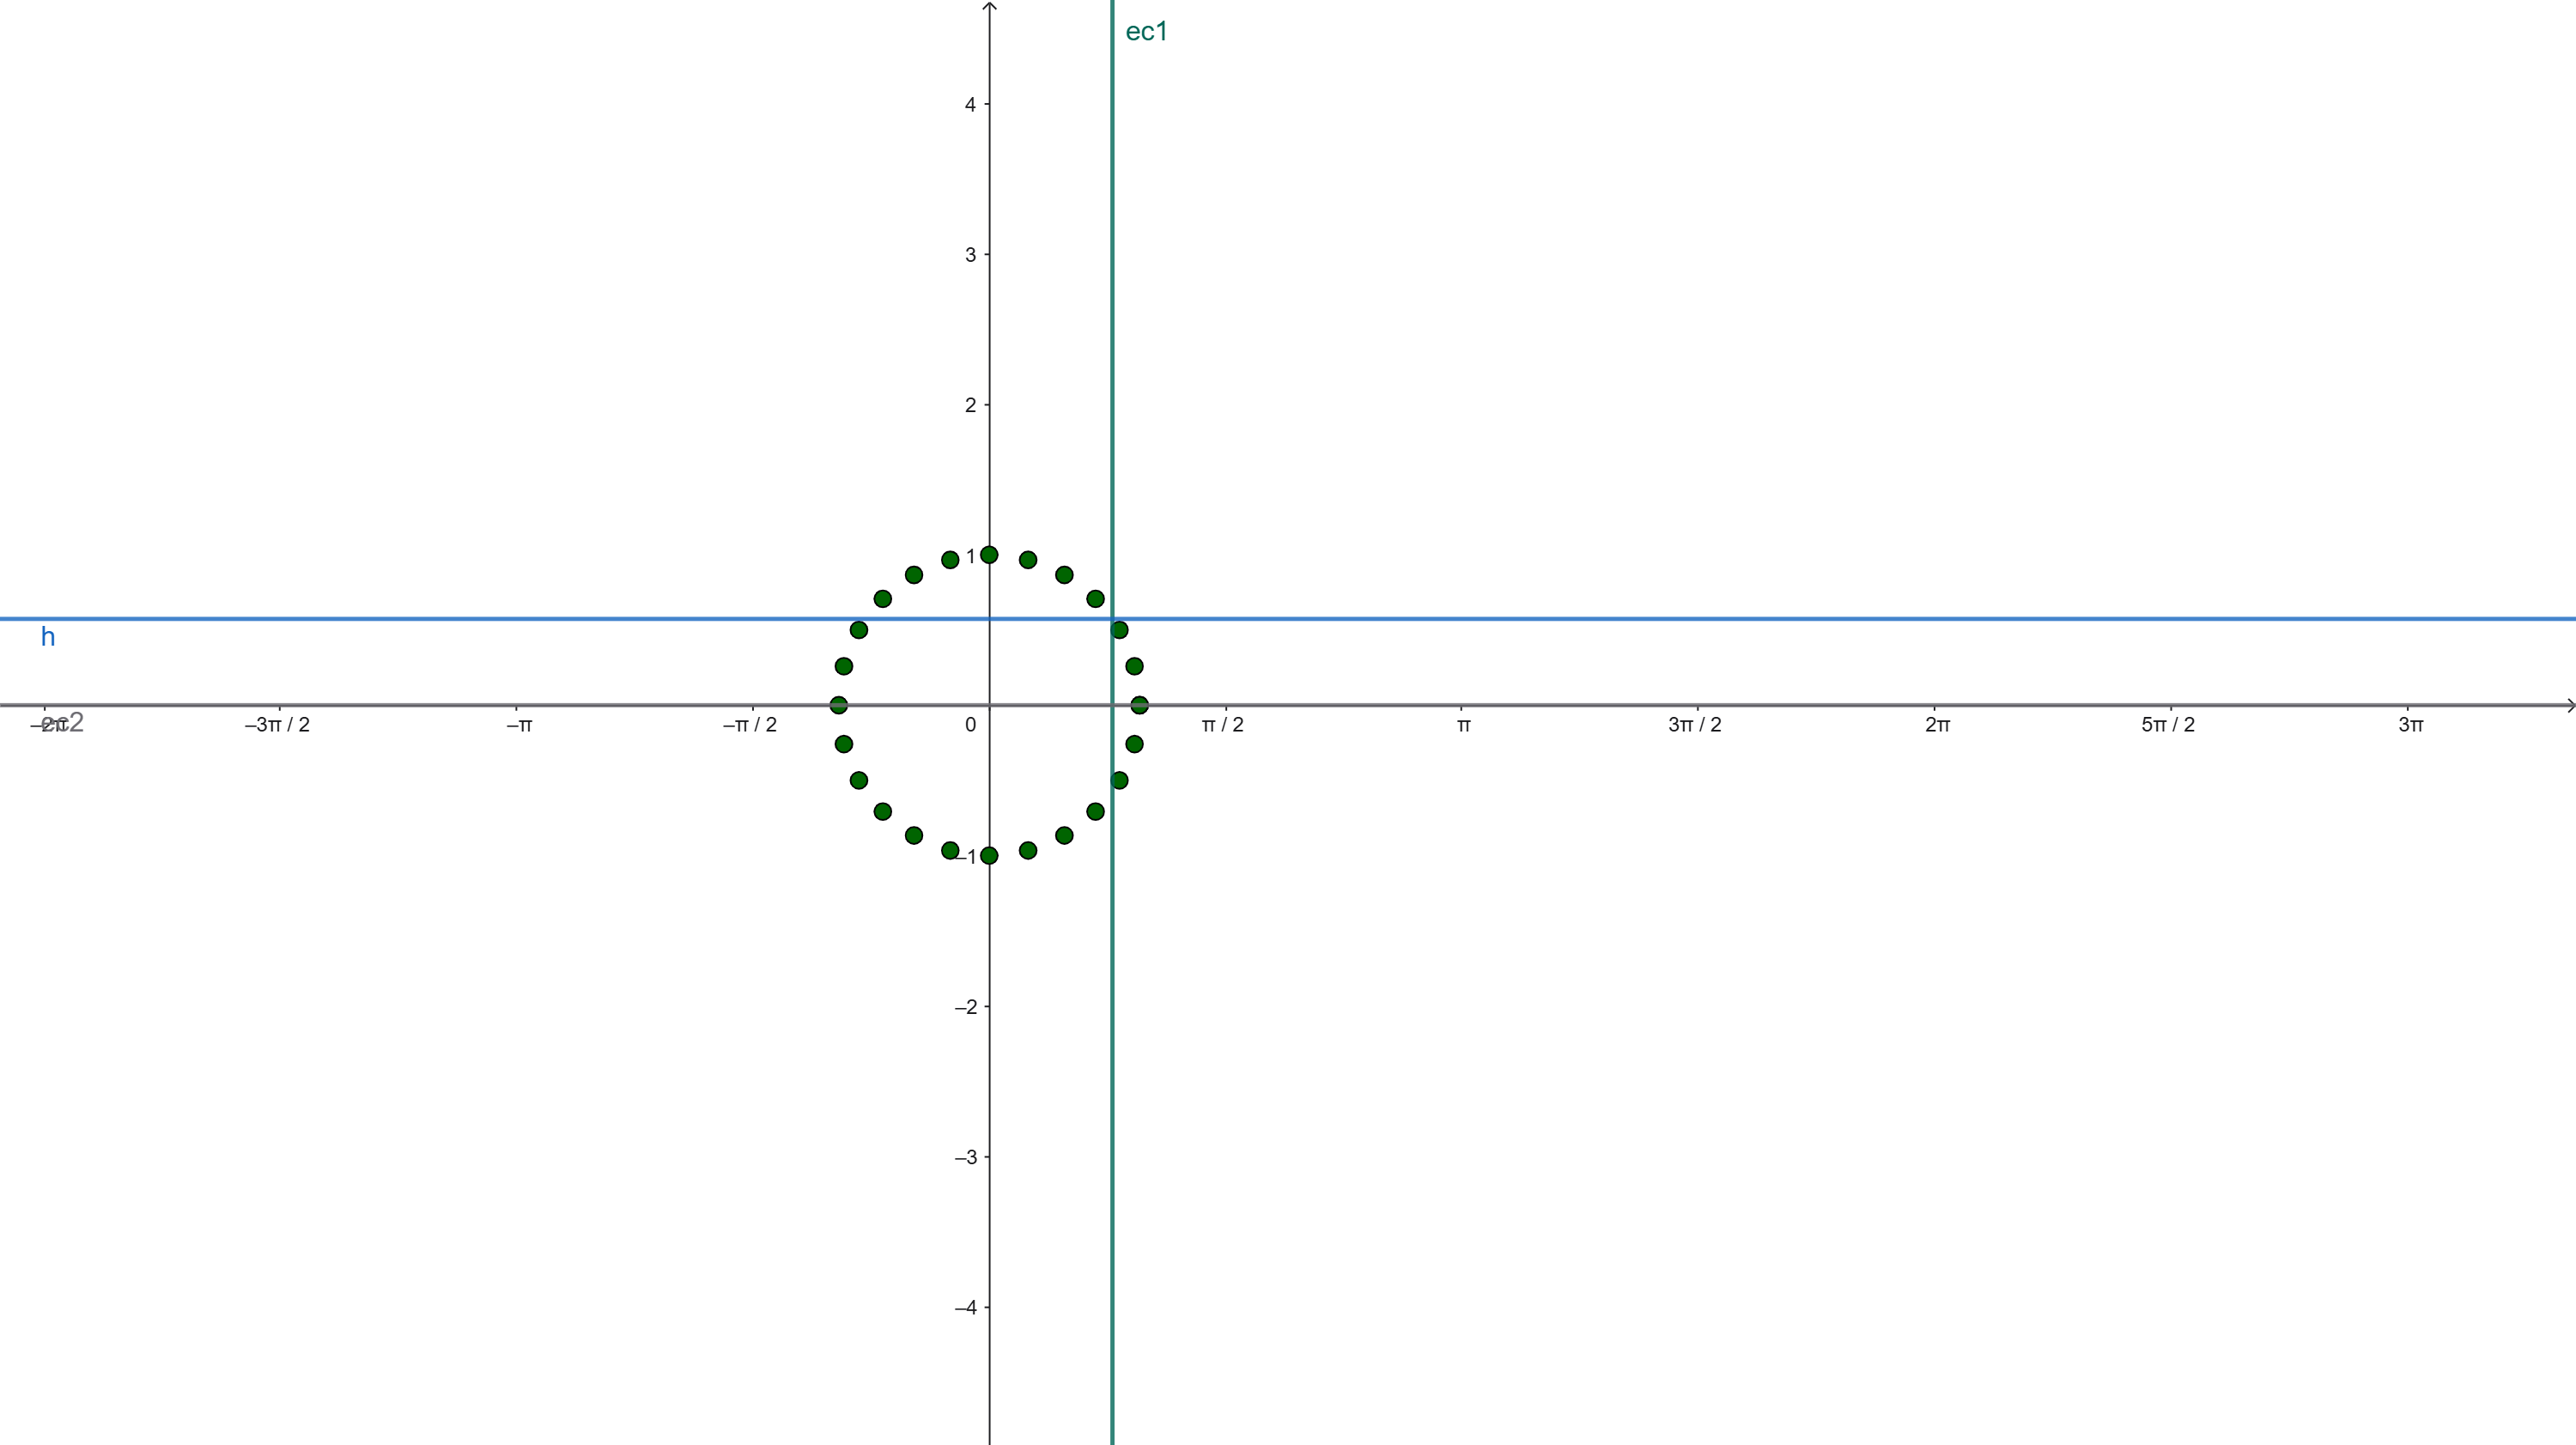
\includegraphics[width=0.55\textwidth]{Apendices/rc.png}
  \caption{Visualización discreta del comportamiento cíclico del tiempo}
  \caption*{GeoGebra: Generación de puntos discretos sobre la circunferencia usando la expresión: \newline
    \texttt{Sequence((cos(2$\pi$ * n / 86400), sin(2$\pi$ * n / 86400)), n, 0, 86400, 3600)}}
  \caption*{La figura incluye dos líneas auxiliares que recorren la circunferencia: una horizontal (coseno) y una vertical (seno), generadas dinámicamente mediante un deslizador \( t \) con paso de 600 segundos. Estas líneas intersectan en el punto \( (x, y) \), representando la posición temporal proyectada en coordenadas trigonométricas.}
  \label{fig:representacion-ciclica-tiempo}
\end{figure}

\begin{figure}[ht!]
  \centering
  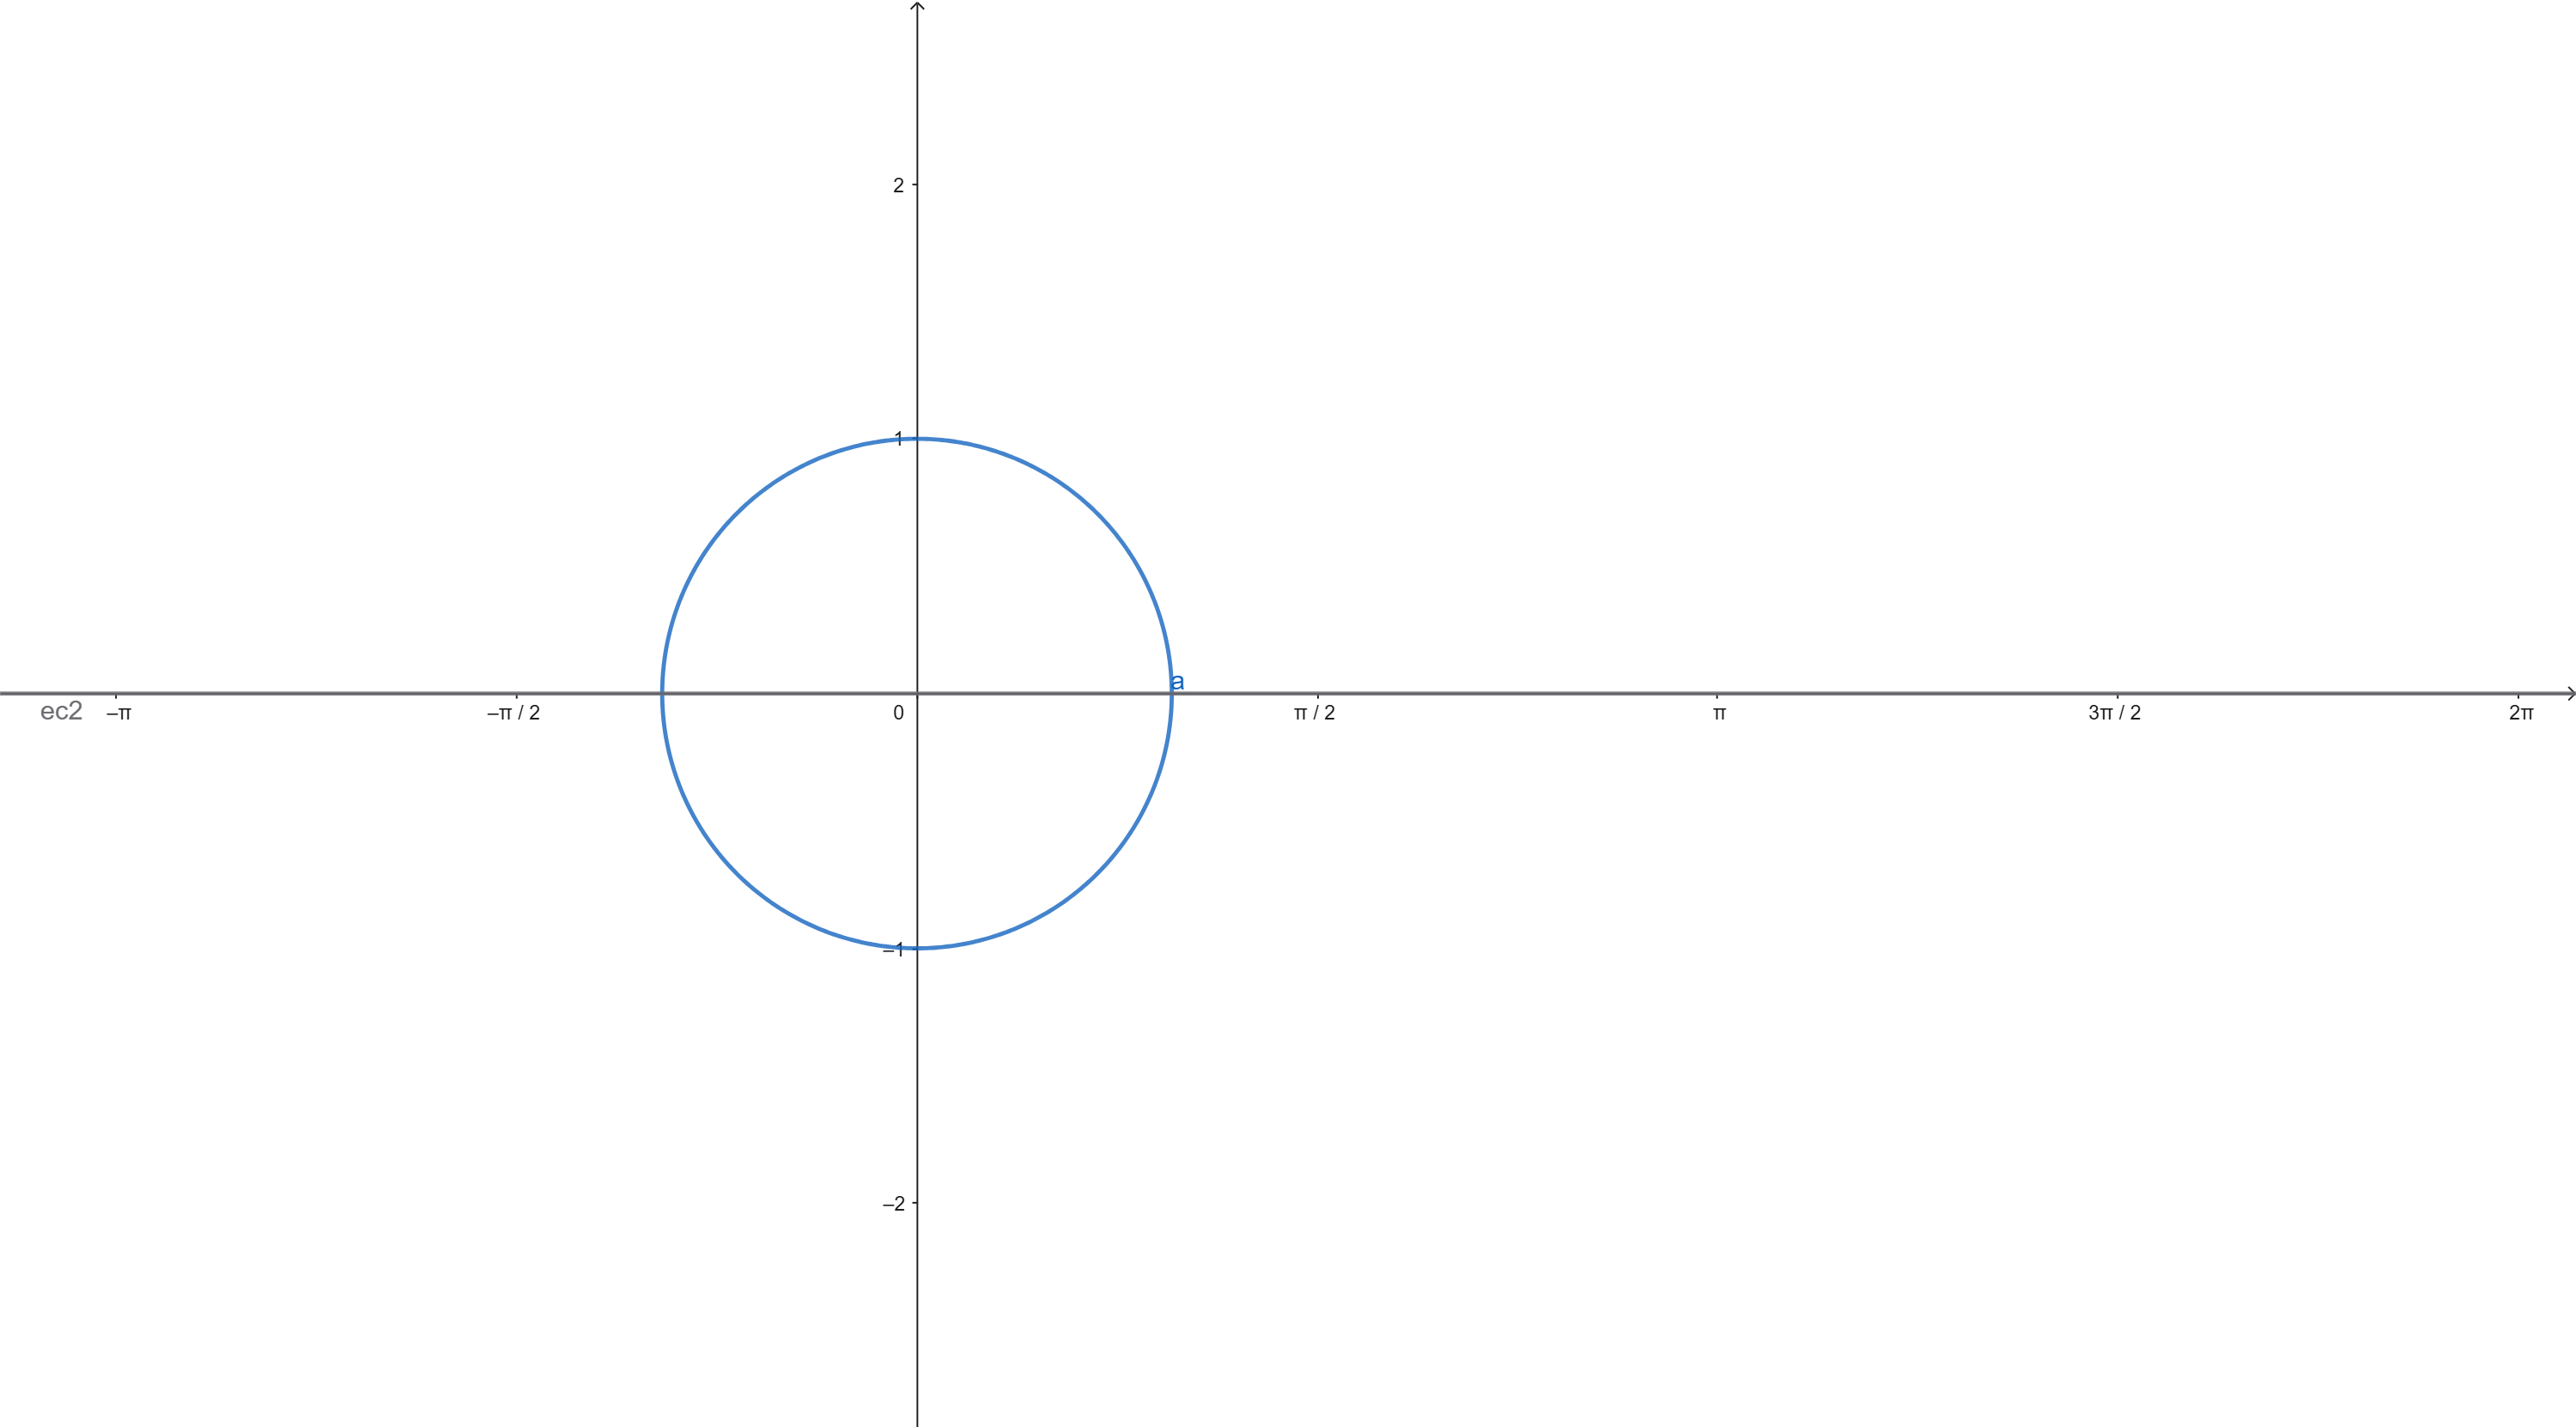
\includegraphics[width=0.55\textwidth]{Apendices/curve.png}
  \caption{Curva paramétrica continua del tiempo sobre el círculo unitario}
  \caption*{GeoGebra: Generación de la curva mediante las expresiones: \newline
    \texttt{x(t) = cos(2$\pi$ * t / 86400)}, \quad
    \texttt{y(t) = sin(2$\pi$ * t / 86400)}, \quad
    \texttt{Curve(x(t), y(t), t, 0, 86400)}}
  \caption*{La figura muestra una curva paramétrica continua que representa el tiempo sobre el círculo unitario mediante funciones trigonométricas. Cada instante se proyecta como un punto único definido por \( x(t) = \cos\left(\frac{2\pi t}{86400}\right) \) y \( y(t) = \sin\left(\frac{2\pi t}{86400}\right) \), donde \( t \) es el número de segundos desde las 00:00. Esta codificación garantiza continuidad angular, permitiendo que modelos de simulación o aprendizaje automático interpreten correctamente la naturaleza cíclica del tiempo sin ambigüedades en los extremos del día.}
  \label{fig:curva-tiempo-circular}
\end{figure}


\uextra{Apendice}{Algorimos de los distintos agentes}
\begin{figure}[ht!]
  \centering
  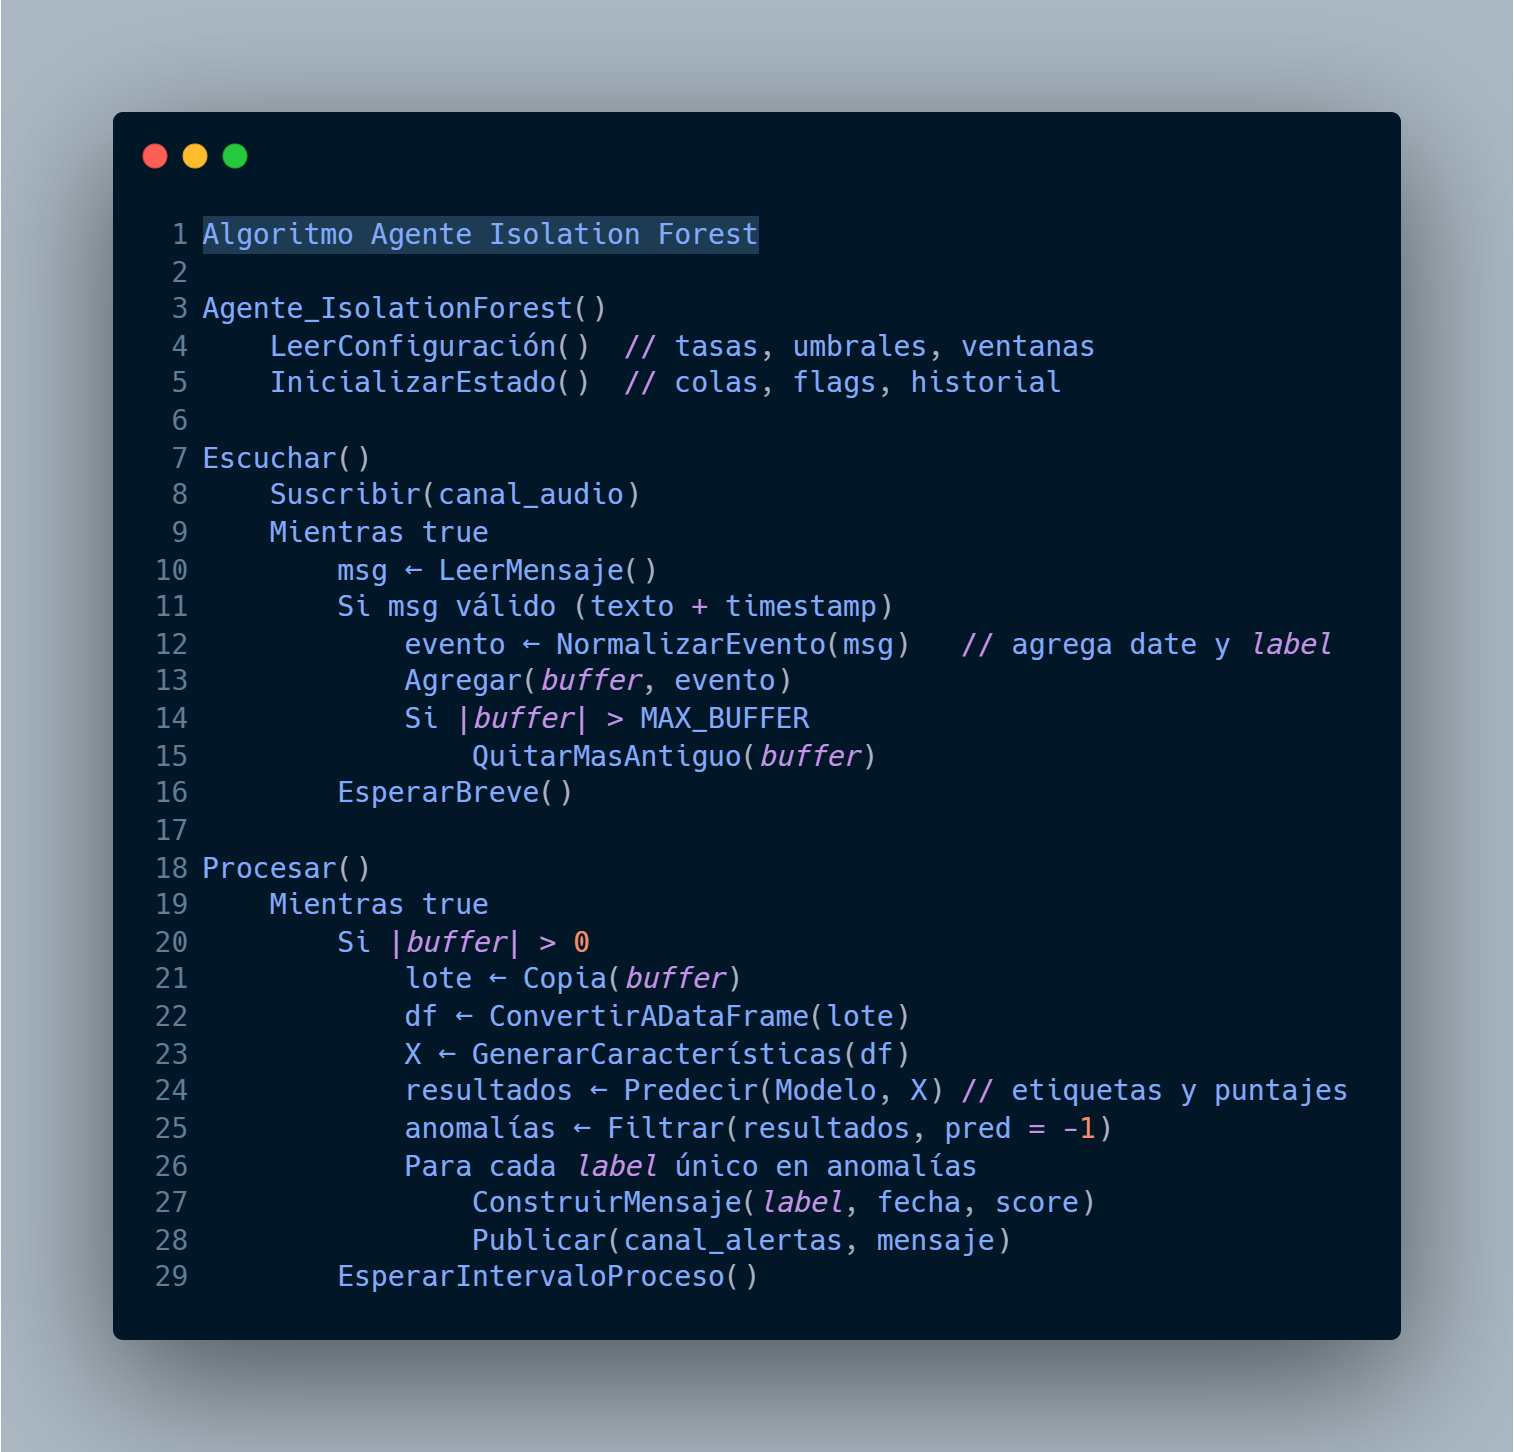
\includegraphics[width=0.95\textwidth]{Apendices/algoritmos/algoritmo_agente_isolation_forest.png}
  \caption{Algoritmo del agente de detección de anomalías basado en Isolation Forest}
  \label{fig:algoritmo_agente_isolation_forest}
\end{figure}

\begin{figure}[ht!]
  \centering
  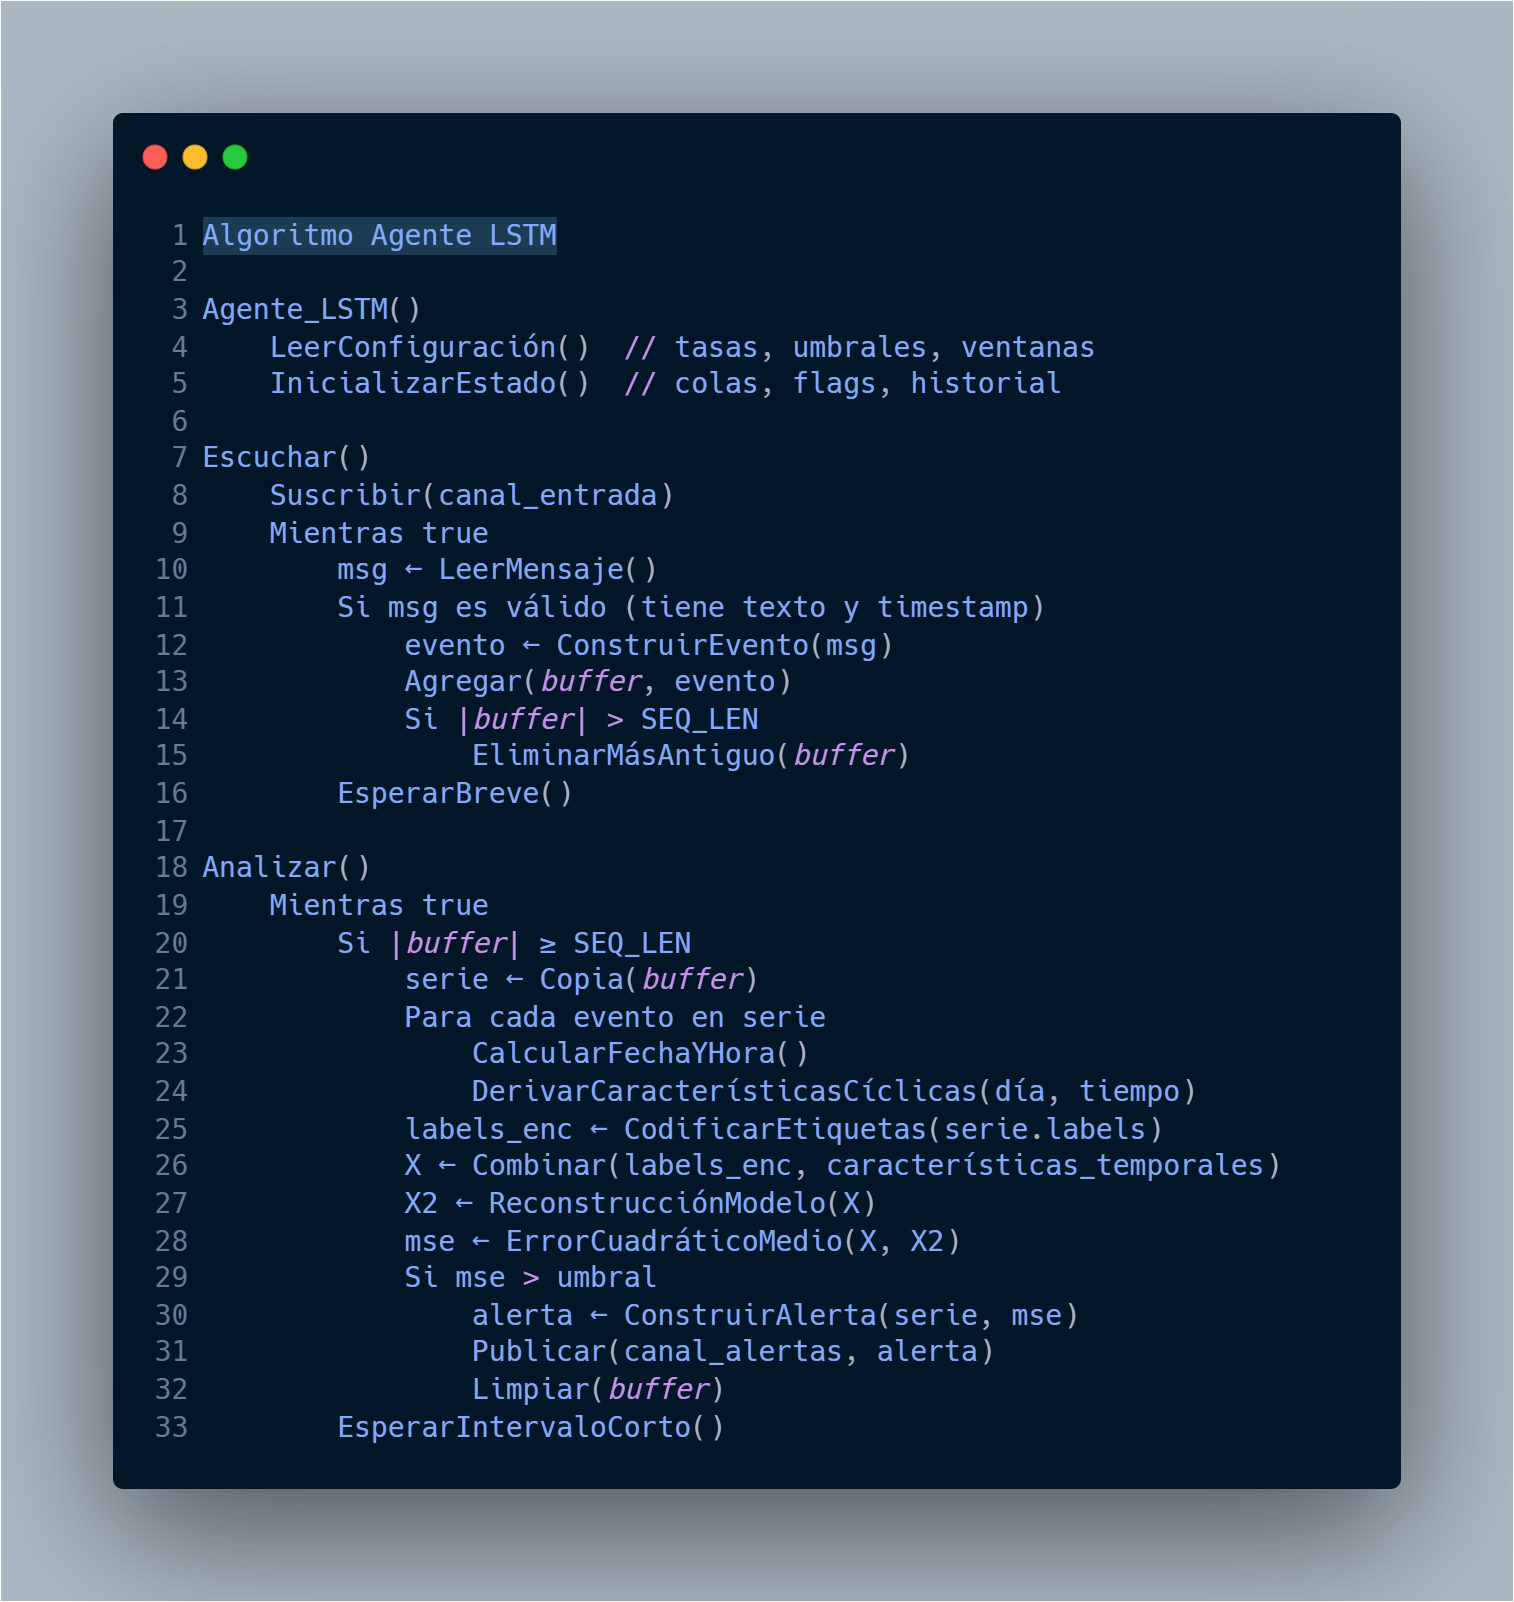
\includegraphics[width=0.95\textwidth]{Apendices/algoritmos/algoritmo_sgente_LSTM.png}
  \caption{Algoritmo del agente de predicción basado en LSTM}
  \label{fig:algoritmo_agente_LSTM}
\end{figure}

\begin{figure}[ht!]
  \centering
  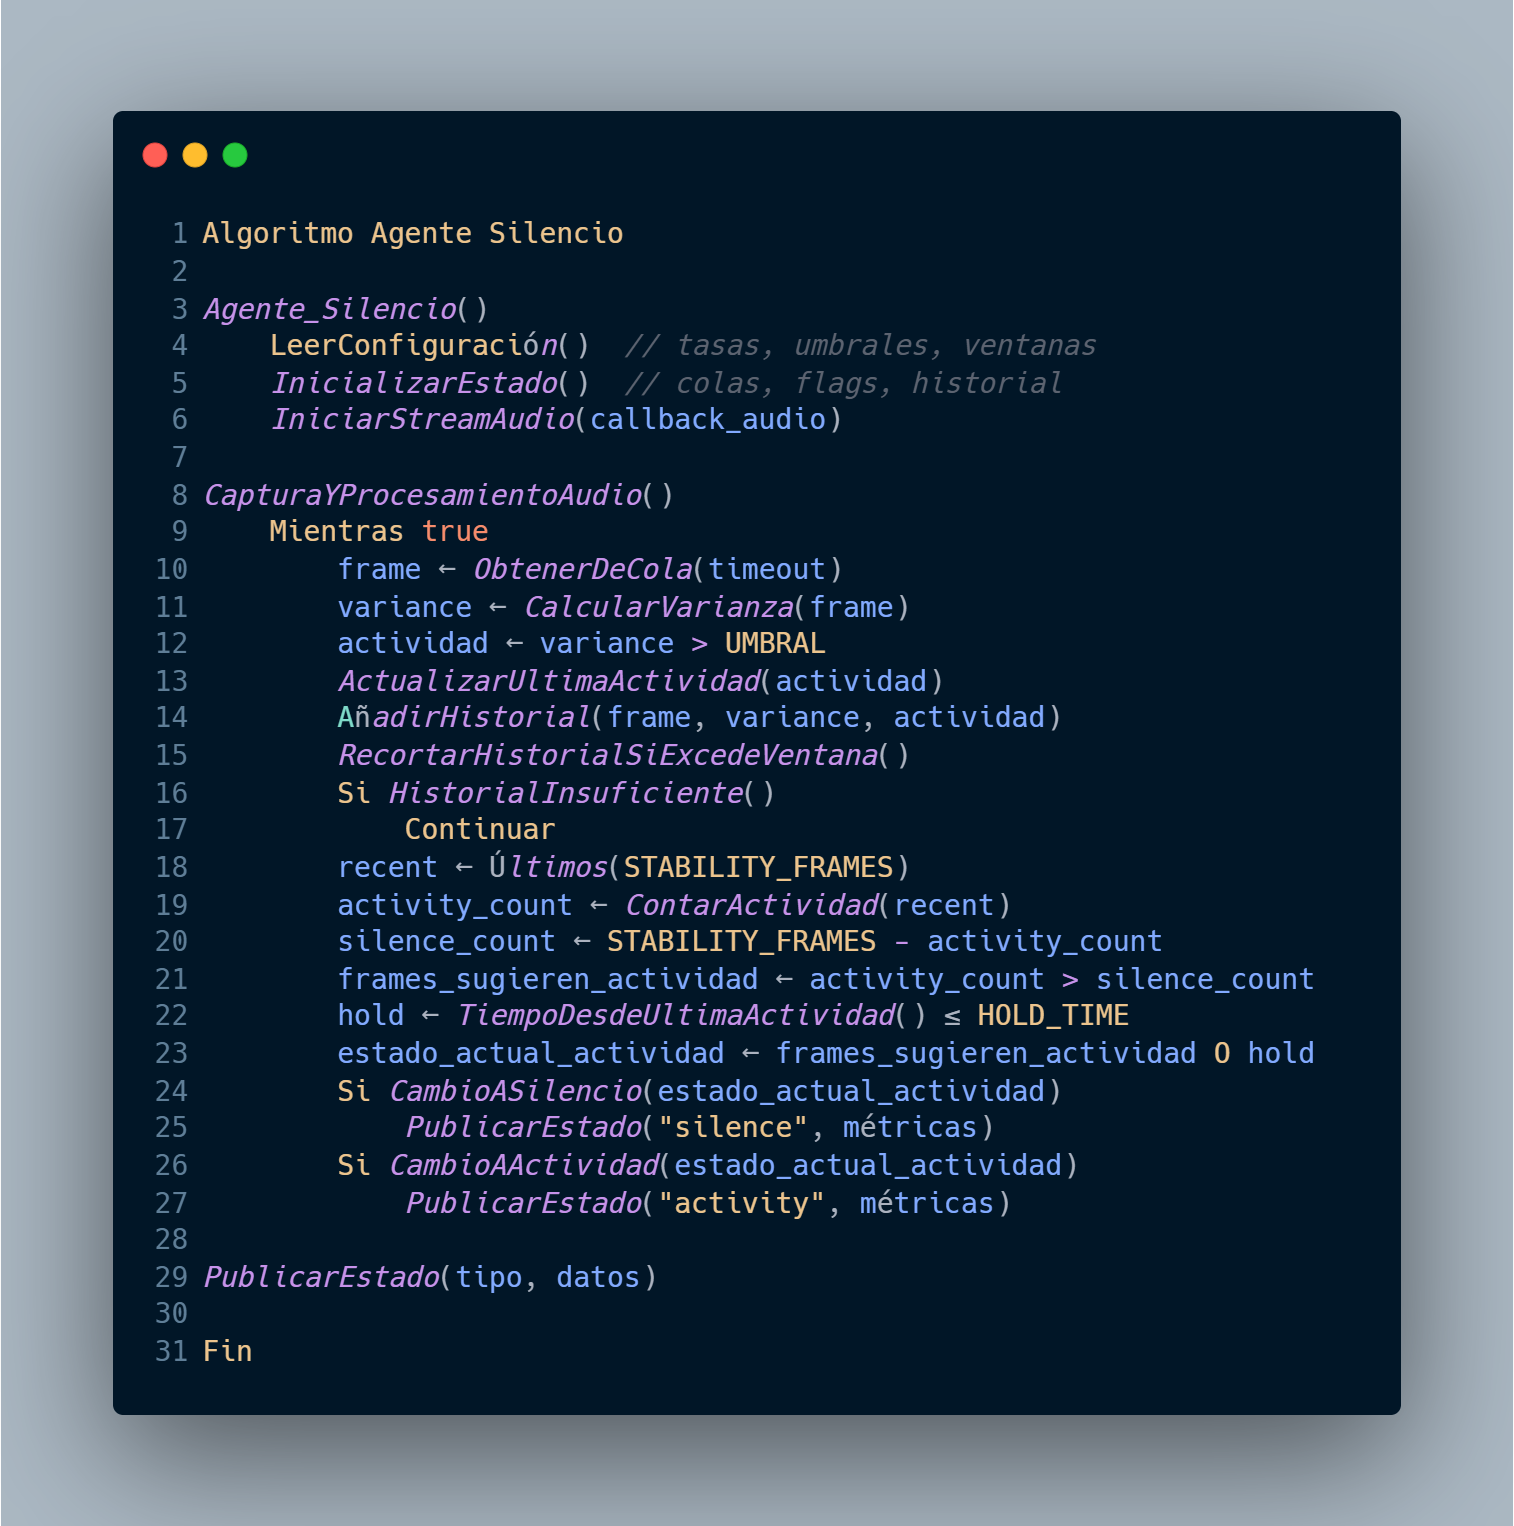
\includegraphics[width=0.95\textwidth]{Apendices/algoritmos/algoritmo_agente_silencio.png}
  \caption{Algoritmo del agente de detección de silencio}
  \label{fig:algoritmo_agente_silencio}
\end{figure}

\uextra{Apendice}{Verificación del sistema de monitoreo acústico}

{\small
  \begin{longtable}[c]{c p{3.5cm} p{2.2cm} p{2.2cm} p{3.5cm}}
    \hline
    \textbf{Requerimiento} & \textbf{Descripción}                                                                                    & \textbf{Entrada}                                                  & \textbf{Salida}                                                       & \textbf{Criterio de Aceptación}                                                       \\
    \hline
    \endfirsthead

    \hline
    \textbf{Requerimiento} & \textbf{Descripción}                                                                                    & \textbf{Entrada}                                                  & \textbf{Salida}                                                       & \textbf{Criterio de Aceptación}                                                       \\
    \hline
    \endhead
    \endfoot
    \endlastfoot

    R1                     & Captura continua del audio ambiental a través de micrófonos.                                            & Señales de audio del entorno a través del hardware del micrófono. & Eventos discretos etiquedados del audio.                              & El sistema debe estar activo y registrando datos en todo momento.                     \\
    \addlinespace
    R2                     & Procesamiento del audio para clasificarlo en eventos sonoros predefinidos.                              & Flujo de datos de audio.                                          & Clasificación del sonido (ej. voz, silencio, golpe).                  & El sistema debe etiquetar correctamente la señal de audio que recibe en todo momento. \\
    \addlinespace
    R3                     & El sistema debe conocer en todo momento el estado de actividad del entorno.                             & Señal de audio.                                                   & Hay ruido o silencio.                                                 & El sistema reconoce cuando hay ruido o silencio.                                      \\
    \addlinespace
    R4                     & Comparación de la actividad en tiempo real con el perfil de normalidad para detectar patrones anómalos. & Secuencia de eventos en tiempo real                               & Identificación de una anomalía o evento atípico.                      & Detectar si una secuencia de eventos es normal o anómala.                             \\
    \addlinespace
    R5                     & El sistema realiza una consulta verbal al usuario al detectar una anomalía.                             & Señal de audio.                                                   & Emisión de una pregunta de voz pregrabada (ej. ``¿Está todo bien?''). & El sistema consulta el estado del usuario antes de enviar una alerta.                 \\
    \addlinespace
    R6                     & Permitir cancelar una alerta de emergencia por comando de voz.                                          & Respuesta de voz del usuario (ej. ``Estoy bien'').                & No se envía alerta.                                                   & El sistema cancela la alerta.                                                         \\
    \addlinespace
    R7                     & El sistema envía notificaciones de emergencia si la anomalía es crítica o el usuario no responde.       & Falta de respuesta del usuario o gravedad de la anomalía          & Envío de notificaciones.                                              & El sistema es capaz de enviar una alerta sin la intervención del usuario.             \\
    \bottomrule
    \addlinespace

    \caption{Requerimientos del sistema acústico}
    \label{tab:requerimientos_sistema_acustico}
  \end{longtable}
}

\uextra{Apendice}{Cuadro comparativo de microcontroladores}

{\small
  \begin{longtable}[c]{p{2.2cm} p{2.4cm} p{2.4cm} p{2.4cm} p{2.4cm} p{2.4cm}}
    \hline
    \textbf{Característica}                                                                                                                                &
    \textbf{Raspberry Pi 4 model B}                                                                                                                        &
    \textbf{NVIDIA Jetson Nano}                                                                                                                            &
    \textbf{Google Coral (TPU)}                                                                                                                            &
    \textbf{Arduino (ej. UNO/Mega)}                                                                                                                        &
    \textbf{ESP32}                                                                                                                                           \\
    \hline
    \endfirsthead

    \hline
    \textbf{Característica}                                                                                                                                &
    \textbf{Raspberry Pi 4 model B}                                                                                                                        &
    \textbf{NVIDIA Jetson Nano}                                                                                                                            &
    \textbf{Google Coral (TPU)}                                                                                                                            &
    \textbf{Arduino}                                                                                                                        &
    \textbf{ESP32}                                                                                                                                           \\
    \hline
    \endhead
    \endfoot
    \endlastfoot

    Capacidad de Cómputo                                                                                                                                   &
    Procesador ARM de alto rendimiento multinúcleo.                                                                                                        &
    Procesador ARM de cuatro núcleos y GPU con 128 núcleos NVIDIA CUDA.                                                                                    &
    Procesador ARM, pero su poder de IA proviene de una TPU especializada.                                                                                 &
    Microcontrolador de 8 o 32 bits.                                                                                                                       &
    Microcontrolador de 32 bits con Wi-Fi y Bluetooth.                                                                                                        \\
 
    \addlinespace
    Memoria y almacenamiento                                                                                                                            &
    2-8 GB RAM, microSD hasta 1 TB                                &
    4 GB RAM, microSD hasta 128 GB                                                                 &
    1 GB RAM, microSD, almacenamiento interno limitado                                                                            &
    2-8 KB RAM, sin almacenamiento persistente                                                                                               &
    512 KB RAM, soporte microSD externo                                                                \\
    \addlinespace
    Costo                                                                                                                                                  &
     65\$ (Amazon)                                                                                                                         &
     165\$ (AliBaba)                                                                                                                &
     144\$                                                                                                                                 &
     27\$                                                                                                                                  &
     Entre 10\$ y 20\$ (Amazon)  
                                                                                                              \\
                                                                                                               \hline
    \caption{Cuadro comparativo de microcontroladores}
    \label{tab:cuadro_comparativo_microcontroladores}
  \end{longtable}
}
